\week{Putting Programs Together}

Last week, we explored how to use \emph{functions} to re-use pieces of rules. From now on, we'll
adopt some new terminology. In the past, we've called everything \emph{rules}, but programmers
actually call these things \term{expressions}. Everything we've seen so far -- numbers, words, functions, and even combinations of them --
is an example of an expression.

Some kinds of expressions have even more particular names. Expressions like \code{+}, \code{-},
and \code{*} are called \term{operators}, to distinguish themselves from the functions we explored
last chapter.

We also learned that computers store everything as numbers -- even graphics! This week, we will
start thinking about what sorts of things we can do with these models. Programs rarely stand
alone. Real programs are built by connecting smaller programs together -- taking the output of one
(or more) thing and feeding it into another.\curious{The technical term for this behavior
is \term{composition}.}  Even though the programs themselves may stay the same, the \emph{stuff}
that flows through them can change. This \emph{stuff} is what computer programmers
call \term{data}.\didyouknow{The word \emph{data} is plural. The singular of \emph{data}
is \emph{datum}, but this very rarely used.}  This is how simple pieces become powerful systems. In
the first week, we saw how complex behavior could be created by a marble rolling through many
machines. This week, we will see something similar -- this time using Python.

But before we do that, we're going to have learn a bit about sound.
\begin{marginfigure}
\label{fig:speaker}
\includegraphics[width=\linewidth]{../week3/figures/loudspeaker.pdf}
\caption{
Schematic of a simple speaker. The computer controls current through the \emph{inductor}, which
causes the inductor coil to magnetize. This pushes or pulls on the static magnet inside the speaker,
which causes the \emph{diaphragm} to move air. This happens thousands of times a second. We perceive
the air movements as sound.
\attribution{By Altavoz.png: Enciclopedia Librederivative work: Flappiefh (talk) - Altavoz.png, CC BY-SA 3.0, https://commons.wikimedia.org/w/index.php?curid=16285077}
}
\end{marginfigure}

\section{A \emph{Note} on Music}

When you hear your favorite song or a symphony orchestra with dozens of instruments or a bird
singing its song or even your little brother banging pots in the kitchen, what you're actually
feeling is the air around your eardrums moving quickly. Sometimes the air pushes them in, sometimes
it pulls them out. Depending on how intense that push and pull is and how often it happens, your
body perceives it as a particular sound.

\begin{figure}[t]
  \fixfigure
  \caption{The relationship between circles, waves, and triangles. A point $A$ is moved around a
    circle of radius $1$ at a constant speed, called the frequency. In this case, the frequency is
    440 times per second or 440 Hz, which corresponds to the middle A of the keyboard. If we plot
    the $y$-value of the point, we get a \emph{sine} wave (the plot of the $x$ value is known as
    \emph{cosine}). Another way to think of \emph{sine} is to draw a triangle between the point
    $O$ (the origin), $A$, and the point on the $x$-axis corresponding to $A$. Then, $\sin(\theta)$ is the same
    as the length of line $o$ over line $h$. This latter relationship holds regardless of whether
    we're dealing with a unit circle (a circle of radius one) or a larger circle. Thus, \emph{sine}
    only really depends on the angle $\theta$, which is why it's written as $\sin(\theta)$.}
  \label{fig:middle-a}
  \centering
  \begin{tikzpicture}[font={\footnotesize\sffamily}, scale=1.4]
  \def\xsize{4}
  \def\cyclecount{3}
  \def\freq{440}
  \def\thetacount{5}
  \pgfmathsetmacro{\dtheta}{((3/4) * pi)/\thetacount}
  \pgfmathsetmacro{\wavelengthms}{(1/\freq) * 1000}
  \pgfmathsetmacro{\sixpioverfive}{((\cyclecount * 2)/\xsize) * pi}
  \def\sincolor{CornflowerBlue}
  \def\circlecolor{Peach}
  \def\xshift{1.5cm + 1em}
  \def\calcthetaparams#1{
    \pgfmathsetmacro{\thetarad}{(#1 - 1) * \dtheta}
    \pgfmathsetmacro{\cy}{sin(\thetarad r)}
    \pgfmathsetmacro{\cx}{cos(\thetarad r)}
    \pgfmathsetlengthmacro{\graphx}{\xshift + ((\dtheta * \thetacount)/(2 * pi) * (\xsize/\cyclecount) * ((#1 - 1) / \thetacount) * 1cm)}

    \pgfmathsetmacro{\dcx}{-\cy}
    \pgfmathsetmacro{\dcy}{\cx}
  }

  \draw[black, <->] (-1.2,0)--(1.2,0);
  \draw[black, <->] (0,-1.2)--(0,1.2);
  \draw[color=lightgray] (0,0) circle (1);

  \foreach \theta in {2, ..., \thetacount} {
    \calcthetaparams{\theta}

  }

  % blue sine wave
  \begin{scope}[xshift=\xshift]
    \draw[step=0.5, lightgray] (0, -1) grid ({\xsize+0.5},1);
    \draw[black, ->] (0,0) -- (\xsize+0.5,0) node[right] {$t$};
    \draw[black, <->] (0,-1) -- (0, 1);
  \end{scope}

  \foreach \theta in {2, ..., \thetacount} {
    \calcthetaparams{\theta}
    \draw[fill=DeepPurple] (\cx, \cy) circle (0.1em);
  }

  \begin{scope}[xshift=\xshift]
    \draw[domain=0:{\xsize+0.5},samples={\cyclecount*30},color=\sincolor, very thick] plot (\x, {sin((\x * \sixpioverfive) r)}) node[right, yshift=-1.1em] {$\sin x$};

    \draw[decorate,decoration={brace, amplitude=5pt, mirror, raise=0.8em}]
       ({\xsize/\cyclecount*1},-1) -- ({\xsize/\cyclecount*2},-1) node[midway,yshift=-2.3em]{\sffamily \footnotesize\begin{tabular}{c}one cycle\\440 cycles per second\end{tabular}};
    \foreach \cycle in {1, ..., \cyclecount} {
      \draw[dashed, very thick, black] ({\xsize/\cyclecount*\cycle}, -1.1) -- ({\xsize/\cyclecount*\cycle}, 1.1) node[above] {\sffamily \footnotesize \pgfmathparse{\wavelengthms * \cycle}\pgfmathprintnumber[fixed,precision=2]{\pgfmathresult}\ ms};
    }
  \end{scope}

  \foreach \theta in {2, ..., \thetacount} {
    \calcthetaparams{\theta}
    \draw[dashed, gray] (\cx, \cy) -- ({\graphx - 0.1em}, \cy);
    \draw[color=DeepPurple, fill=DeepPurple] (\graphx, \cy) circle (0.1em); % --[dashed, color=lightgray]
  }

  \calcthetaparams{2}
  \draw[black] (\cx, \cy) node[above, right, yshift=0.5em] {$A$};
  \draw[black,->] ({\cx * 1cm + (0.11em * \dcx)}, {\cy * 1cm + (0.11 * \dcy)}) -- ({\cx * 1cm + (1em * \dcx)}, {\cy * 1cm + (1em * \dcy)});

  \draw[black] (0, 0) node[xshift=-0.6em,yshift=-0.6em] {$O$};
  \calcthetaparams{3}
  \draw[dashed,black] (0,0) -- (\cx, \cy) node[midway, yshift=0.5em, xshift=-0.5em, black] {$h$} -- (\cx, 0) node[midway, right, xshift=-0.2em, yshift=-0.7em] {$o$};

  \draw[black] (1em,0) arc[start angle=0, end angle={deg(\thetarad)}, radius=1em] node[right, midway, yshift=0.3em, xshift=-0.3em] {$\theta$};

  \foreach \y in {-1, ..., 1} {
    \node[black, left] at ({\xshift -0.5em}, \y) {\sffamily \y};
  }

\end{tikzpicture}

\end{figure}

Notice I said push and pull, if the air kept pushing or kept pulling, your ears would get
hurt. Thus, the air has to be moved back \emph{and} forth.

Headphones, speakers, musical instruments, and your vocal cords contain vibrating surfaces that push
and pull air. As the air is moved in these places, it causes the air outside to move as well, and
the sound travels towards the hearer.

A speaker is made up of a thin membrane called a diaphragm. The computer sends it a signal that
specifies how much to push or pull the diaphragm. When done quickly this causes the air to
move. This is done using a \term{sound card}, a special computer component that converts numbers in
a system like Python into an electrical signal that can move a speaker.

To make a computer play a sound from Python we have to produce a lot of numbers that correspond to
how much to move the diaphragm. The amount of times we have to do this per second is known as
the \term{sampling rate}. The most common sampling rate ued today is 44100 Hz or 44.1 kHz.\didyouknow{The symbol
Hz stands for ``Hertz'' which is a unit that means the number of times per second something
happens. If a juggler threw two balls into the air every second, they would be throwing balls at a
rate of 2 hertz. The prefix ``k'' stands for kilo, which is a Greek word meaning one thousand. A
juggler juggling at the rate of 2 kilohertz would have to be going very fast!}

But what numbers do we have to produce? This requires a bit of technical musical knowledge, but for
our purposes the note corresponding to ``middle A'' is usually taken to be the sound that would be
made by something vibrating back and forth at a rate of 440 Hz
(see \prettyref{fig:middle-a}).

\subsection{Producing our first note}

Let's begin by importing the modules for this class.

\begin{replbox}
from week3.examples as *<ENTER>
import week3.synth as synth<ENTER>
\end{replbox}

The first thing we want to do is open up our waveform viewer. This will show us the
actual \term{samples} (speaker diaphragm offsets) being sent to the speakers.

\begin{replbox}
synth.view(synth.note('A1'))
\end{replbox}
\hint{A4 refers to middle A. A5 refers to the A one octave above middle A, and A3 the octave below.}.

If you zoom in, you can see how the wave changes back and forth to produce the note.

You can look at two notes side by side as well. Let's look at two notes that sound good together.
\begin{replbox}
synth.view(synth.note('A4'), synth.note('E4'))
\end{replbox}
\curious{What do you notice about the number of times the E wave repeats versus the number of times the A one does?}

Now let's look at an octave
\begin{replbox}
synth.view(synth.note('A4'), synth.note('A5'))
\end{replbox}

You can also supply frequencies directly:
\begin{replbox}
synth.view(synth.note(440), synth.note(880))
\end{replbox}
\huh{You said sound waves are continuously moving air back and forth
but the computer only moves the speaker diaphragm 44 thousand times each second. That's not
continuous!}{You're right. The speaker diaphragm is moved in bursts 44100 times each second. A
mathematics theorem, called the Whittaker-Nyquist-Shannon theorem after its discoverers, says you
can reconstruct a continuous signal from a digital representation with a sampling rate twice the
highest pitch. The highest pitch a human can hear is about 20kHz. Thus, the choice of 44.1 kHz means
that the speaker can actually reconstruct the full signal. Amazing!}

Let's try sending the note to the sound card:
\begin{replbox}
synth.play(synth.note('A4'))
\end{replbox}

\subsection{Timbre}

But it can't be that simple right? After all, if this simple wave is the middle A, why does a piano
sound diferent from a trombone from a violin? Surely there's more going on? If you thought this,
you'd be correct. There is a lot more going on. The simple wave we saw above is the simplest
possible wave,\curious{The term \emph{sine} is a word from trigonometry and has to do with angles of
a triangle and ultimately with a circle. These three shapes may seem to have nothing to do with one
another, but they are intimately connected, as shown in \prettyref{fig:middle-a}.} but no
real life sound wave looks like this. Instead, real life waves have a ``shape'' known as the
\term{timbre}. Any shape of wave that repeats the same number of times per second will seem to produce the
same pitch to our ears, but the shape causes us to perceive a different ``color'' or ``timbre'' of
sound.

Let's see if we can add some timbre to our notes.

\section{Transforming Sound}

Just like we saw at the start of class, we can start with a simple tone and make new sounds by
adding materials that transform the original sound. Similarly, we can transform sound on the
computer. When multiple tones sound off at the same time, that creates a different timbre. We can
manipulate tones by changing volume or adjusting frequency.

\hint{Anything appearing after a
    \code{\#} in Python is treated as a \term{comment}, which means
    that it's just there for someone reading the code.}
\begin{TryThisBox}
  Try creating a new instrument in a function in
  \texttt{week3/instruments.py}
\begin{lstlisting}
def myinstrument(note, t):
  t1 = synth.tone(note, t)
  t2 = synth.tone(note * 2, t)
  t3 = synth.tone(note * 3, t)
  # Multiplying t1 and t2 change the volume of the tones
  return (8/10) * t1 + (2/10) * t2 + (1/20) * t3
\end{lstlisting}
\end{TryThisBox}

\mTrackBox{Music \& Sound}{Instruments make noise by vibrating air using strings, membranes, or open tubes. The
  construction of the instrument generates the timbre produced and the exact harmonics that get
  sounded and how loud those harmonics are. The instrument body acts as a resonator, which is a
  fancy way of saying it further modifies the volumes of those frequencies.

  The harmonics we introduced above are easiest to understand on stringed instruments. A string
  instrument makes a noise by vibrating a string. When you vibrate a string at a given frequency,
  the only waves that can ``stand'' on that string are waves whose frequencies are integer multiples
  of the frequency that string is tuned to. This is illustrated by the diagram below.
  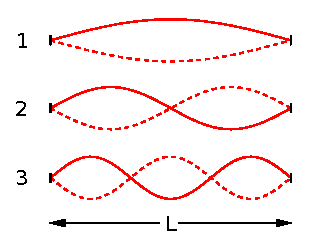
\includegraphics[width=0.9\linewidth]{../week3/figures/standing-waves.eps}
  \attribution{MikeRun, CC BY-SA 4.0 <https://creativecommons.org/licenses/by-sa/4.0>, via Wikimedia Commons}
}
Now play this, and see what happens. That tone sounds more complex already!

What happened here? This is the first time we're seeing the usage of \code{=}. The equals makes a
name, like \code{t1}, refer to the result of Python evaluating the expression to the right hand
side. These names are called \term{variables}. If we had just played \code{t1}, we would have gotten
the simple tone we heard above. But by giving the tone a name, and then naming \code{t2}, we are able
to manipulate the waveforms.

Adding tones like this is called adding \term{harmonics}. Harmonics increase the complexity of the
sound and arise naturally when an instrument is sounded.

\begin{BigIdeaBox}
We can use \code{=} to capture data as names called \emph{variables} and then re-use these later on
\end{BigIdeaBox}

\subsection{Coloring our Notes}
\label{subsec:coloring-our-notes}

Above, the volume and pitch were \term{static}, which means that they didn't change over time. We
can also adjust these slightly for some cool effects. These add \emph{color} to the notes, which add
musicality.

The first is tremolo, which comes from changing the \emph{volume}, which is controlled by how
\emph{big} the wave is.

\begin{TryThisBox}
  \begin{lstlisting}
def tremolo(note, t):
  tremolo = synth.tone(10, t)
  volume = 1 + tremolo * 0.1
  return volume * synth.tone(note, t)
  \end{lstlisting}
\end{TryThisBox}

Let's break down each part of this.
\hint{It's important to understand that even though our \code{myinstrument} function remains the same, the data flowing through it are changing constantly as time changes. The fact that we can describe changing things with an unchanging description is one of the coolest parts of programming!}

\begin{figure}[p]
  \fixfigure
  \centering
  \begin{subfigure}{0.9\textwidth}
    \caption{Base Wave}
    \includegraphics[width=\textwidth]{../week3/figures/tremolo-base.pdf}
    \label{subfig:tremolo-wave-basic}
  \end{subfigure}
  \hfill
  \begin{subfigure}{0.9\textwidth}
    \caption{Transformed}
    \includegraphics[width=\textwidth]{../week3/figures/tremolo-transformed.pdf}
    \label{subfig:tremolo-wave-transformed}
  \end{subfigure}
  \hfill
  \begin{subfigure}{0.9\textwidth}
    \caption{Transformed and shifted}
    \includegraphics[width=\textwidth]{../week3/figures/tremolo-final.pdf}
    \label{subfig:tremolo-wave-final}
  \end{subfigure}

  \caption{A comparison of the tremolo waveforms: (a) illustrates the base waveform generated
  by \code{tone(6,t)} which ranges from $-1$ to $1$, (b) shows after our scaling transformation, and
  (c) shows the tremolo effect after shifting up and the result of multiplying it over a base wave
  form (dotted line).}

  \label{fig:tremolo-wave}
\end{figure}

Firstly, we calculate \code{tremolo}. This results in a wave like in
\prettyref{fig:tremolo-wave} (subfigure (a)). The wave peaks at 1 and
troughs at $-1$ (peak and trough is a fancy way of saying the highest
and lowest points).

Volume can't be less than zero, because there's no such thing as being quieter than
silence. Therefore, we have to \emph{transform} the wave, which means we have to move it into the
right position.

In this case, we want the range of volumes to go between $0.9$ and $1.1$. This is our choice; you
can (and should) make your own choice. In order to get to that range, we first \emph{scale} the wave
by the total difference between our chosen high and low points, which is $0.2$. Thus we
get \code{tremolo * 0.2}. But wait! The scale of the original wave itself is also 2, because the
distance between its trough of $-1$ and its peak of $1$ is 2. Thus, we have to \emph{divide} also by
2. Thus, we have \code{tremolo * 0.2 / 2} which is the same as \code{tremolo * 0.1}.

If we plot this (see (b) in \prettyref{fig:tremolo-wave}), we see that the trough is now $-0.1$
and the peak is $0.1$. We want our volume range to be between $0.9$ and $1.1$, which means we have
to \emph{offset} it by $1$, which is the distance between the $-0.1$ and $0.9$ or the distance
between $0.1$ and $1.1$.

Let's try playing this tone. What does it sound like?

\begin{replbox}
  synth.play(tremolo, synth.note('A4'))<ENTER>
\end{replbox}

Another way to modify the tone of a note is \emph{vibrato} which is
when the pitch of a note is shifted back and forth over
time.\didyouknow{Violinists and other string players accomplish this
  by jiggling their fingers back and forth over the string to increase
  and decrease the length of the string}.

Here's an example:

\begin{TryThisBox}
  \begin{lstlisting}
def vibrato(note, t):
  vibrato = synth.tone(6, t)
  return synth.tone(note + vibrato * 0.002, t)
  \end{lstlisting}
\end{TryThisBox}

Try playing this:

\hint{The third argument to \code{synth.play} affects how long the note is played for}
\begin{replbox}
  synth.play(vibrato, synth.note('A4'))<ENTER>
  synth.play(vibrato, synth.note('A4'), 60)<ENTER>
\end{replbox}

Do you notice anything about the second note? You may hear the vibrato become stronger and stronger
as time goes by. This is due to some complicated mathematics, but it is unfortunately noticeable if
we were to use this instrument in real life. But we can get around it. Here's how.

\begin{TryThisBox}
  \begin{lstlisting}
def vibrato(note, t):
  vibrato = @@synth.vibrato_phase(6, t)@@
  return @@synth.tone_from_phase(note * t + vibrato * 0.002)@@
  \end{lstlisting}
\end{TryThisBox}

Without getting too much into the mathematical detail, we get around this by using the
\code{tone\_from\_phase} function which produces a note given a \emph{phase}. A phase is simply
``where'' along the time axis you are (see the graph for middle A \prettyref{fig:middle-a}). The
\code{synth.tone(pitch, t)} calculated the phase for you inside, but when using vibrato, we have to
calculate it separately and adjust the phase directly.

This brings up another good point about functions: we have to think carefully about which arguments
we accept. While it may seem easy to just allow the simplest arguments that make sense, sometimes we
have to allow users to have more flexibility for how they use\curious{Computer programmers often say
  the \term{call} a function.} our function. In this case, the \code{synth.tone} doesn't have the
proper arguments to get the behavior that we need for vibrato.

Now, try hearing the tone again. Much better this time!

\begin{replbox}
  synth.play(vibrato, synth.note('A4'), 60)<ENTER>
\end{replbox}

\subsection{Building our own instruments}

\begin{table*}[t]
  \fixfigure
  \label{tab:synths}
  \caption{More functions you can use to manipulate instrument voices. Pay attention to the arguments to the functions.}
  \footnotesize
  \begin{tabular}{p{0.2\textwidth}p{0.7\textwidth}}
    \toprule
    Function Name & Description \\ \midrule
    \code{tone(pitch, t)} & Produces a simple sine wave of the given pitch (in Hertz) \\
    \code{tone\_from\_phase(p)} & Produces a wave from a \emph{phase} (see \prettyref{subsec:coloring-our-notes}) \\
    \code{vibrato\_phase(r, t)} & Produces a vibrato \emph{phase} (see \prettyref{subsec:coloring-our-notes}) that beats \code{r} times each second \\
    \code{fade\_in(t)} & Produces a \emph{linear} fade-in effect starting at time 0 and ending at time 1 going from silence to full volume \\
    \code{adsr(a, d, t)} & Produces an \emph{attack, decay, sustain, release} envelope for your instrument. The attack and decay segments take \code{a} and \code{d} seconds respectively \\
    \code{rectify(w)} & Adds some ``brightness'' or ``organ''-ness to a sound \\
    \code{soft\_clip(w)} & Adds a ``jazz-organ''-ness to a sound. Sort of cartoony and bubble-y\\
    \code{hard\_clip(w)} & Adds a small ``tinny''-ness to a sound \\
    \code{pluck(t)} & Short ``pluck'' envelope for a sound \\
    \bottomrule
  \end{tabular}
\end{table*}

As we discussed above, when a note is played on a real instrument, we hear a tone for that
note \emph{as well as} all multiples of that pitch. This is what physics tells us \emph{ought} to
happen. However, in real instruments, things are not perfect: piano wires are not perfect strings
and flutes are not perfect tubes. Thus, the harmonics are slightly off pitch. Moreover, different
harmonics fade faster than others and some harmonics may maintain effects like tremolo and vibrato
longer than others. Using the functions in \prettyref{tab:synths} we can build a wide variety of
these effects.

Let's start with a simple ``real'' instrument.  \didyouknow{Fractions
  show up everywhere in music. The intervals between notes correspond
  to particular ratios of their frequencies. For example, the ratio of
  a note one octave above another note is exactly two. So if middle A
  is 440 Hz, then the A one octave above is 880 Hz. Similarly, a note
  a \emph{perfect fifth} above is $\frac{3}{2}$ the frequency of the
  lower note. You can construct the entire 12-tone chromatic scale by
  walking the circle of fifths and applying this ratio as you go up
  and down the circle, while adjusting for octave.

  \includegraphics[width=0.9\linewidth]{../week3/figures/circle-of-fifths.pdf}
  \attribution{User:Jtir, CC BY-SA 3.0 <http://creativecommons.org/licenses/by-sa/3.0/>, via Wikimedia Commons}
}

\begin{TryThisBox}
\begin{lstlisting}
def simple1(note, t):
  # Produce tones that are the fundamental frequency, but with some adjustment so they're off pitch
  t1 = synth.tone(note * 0.997, t)
  t2 = synth.tone(note * 1.001, t)
  fundamental = t1 + t2

  harmonic1 = synth.tone(note * 2.01, t)
  harmonic2 = synth.tone(note * 3.05, t)
  harmonic3 = synth.tone(note * 4.001, t)

  # Adding the waves together, the peaks and troughs can sum up to a max of 5
  return (fundamental + harmonic1 + harmonic2 + harmonic3) / 5
\end{lstlisting}
\end{TryThisBox}

Here we take the tone, adjust it a bit to make it \emph{slightly} off pitch. Then we add harmonics,
but instead of multiplying by $2,3,4,\ldots$ we multiply by slightly different numbers. In this
case, all the harmonics are slightly higher or \emph{sharp}. This produces a sort of pitch more like
a piano, whose harmonics are all sharp.

% TODO is it messy?
One thing you may hear is that this tone sounds ``messy''. This is because we weigh each harmonic
the same. As we add harmonics together, we note that, since each harmonic wave ranges from $-1$ to
$1$, adding together five of them can lead to a wave ranging from $-5$ to $5$. Thus we divide by 5.

However, if we weigh the harmonics, so that higher harmonics are ever quieter than the fundamental
tone, we get a more realistic sound.

\begin{TryThisBox}
\begin{lstlisting}
def simple2(note, t):
  t1 = synth.tone(note * 0.997, t)
  t2 = synth.tone(note * 1.001, t)
  fundamental = t1 + t2
  harmonic1 = synth.tone(note * 2.01, t)
  harmonic2 = synth.tone(note * 3.05, t)
  harmonic3 = synth.tone(note * 4.001, t)
  return (fundamental + # weight 2
      0.4 * harmonic1 + # weight 0.4
      0.1 * harmonic2 + # weight 0.1
      0.08 * harmonic3 # weight 0.08
      ) / 2.58 # divide by total weight
\end{lstlisting}
\end{TryThisBox}

This sounds a bit more realistic, but you may note that, unlike a real piano, this tone continues
forever. A real piano tone decays over time as the string becomes quieter due to not being hit
anymore. This is characteristic of percussion instruments.

Let's add this to our instrument

\begin{TryThisBox}
\begin{lstlisting}
def simple3(note, t):
  # Example of decay
  t1 = synth.tone(note * 0.997, t)
  t2 = synth.tone(note * 1.001, t)
  fundamental = t1 + t2
  harmonic1 = synth.tone(note * 2.01, t)
  harmonic2 = synth.tone(note * 3.05, t)
  harmonic3 = synth.tone(note * 4.001, t)
  sustained_note = (fundamental + # weight 2
      0.4 * harmonic1 + # weight 0.4
      0.1 * harmonic2 + # weight 0.1
      0.08 * harmonic3 # weight 0.08
      ) / 2.58 # divide by total weight
  return fade_out(t) * sustained_note
\end{lstlisting}
\end{TryThisBox}

\hint{Try replacing the fade in \code{simple3} with an exponential fade by looking at \prettyref{tab:synths}. Does it sound different to you?}
In \code{simple3} we keep everything the same, except we multiply the final wave
by \code{fade\_out(t)}. This function starts at $1$ and then goes eventually to zero. There are
different kinds of fade. Another fade is called an \emph{exponential} fade, which fades out faster.

You can also fade out higher harmonics more quickly than the lower one. This is how real instruments
like pianos sound, because higher frequencies decay faster. How can we fade something out \emph{more
quickly}?

\begin{TryThisBox}
\begin{lstlisting}
def simple4(note, t):
  # Example of decay
  t1 = synth.tone(note * 0.997, t)
  t2 = synth.tone(note * 1.001, t)
  fundamental = @@(t1 + t2) * fade_out(t)@@
  harmonic1 = synth.tone(note * 2.01, t) @@ * fade_out(1.5*t)@@
  harmonic2 = synth.tone(note * 3.05, t) @@ * fade_out(2 * t)@@
  harmonic3 = synth.tone(note * 4.001, t) @@ * fade_out(10 * t)@@
  return (fundamental + # weight 2
      0.4 * harmonic1 + # weight 0.4
      0.1 * harmonic2 + # weight 0.1
      0.08 * harmonic3 # weight 0.08
      ) / 2.58 # divide by total weight
\end{lstlisting}
\end{TryThisBox}

\curious{There's a \emph{lot} more to simulating the sound of a real piano. Real pianos start out with lots of harmonics that are very off pitch and slowly, these harmonics disappear to make way for ever purer tones. That's why piano notes seem to ``develop'' over time. Great pianists can control the development by how they strike the keys. The sound of other notes nearby can also re-excite different harmonics of a pressed key leading to ever developing sound.}

In \code{simple4} we multiply each harmonic separately by \code{fade\_out} and the higher harmonics
have a \code{fade\_out} where the time \code{t} is multiplied by a number. This makes time appear to
run faster for this \code{fade\_out}, so the tone fades out quicker. How does that sound to you?

Multiplying tones like this so that their volume fades over time is known as placing them in
an \term{envelope}. This is because the volume function that we may has the visual effect of
``enveloping'' the inner wave.

There's still something lacking about this though. The tone seems to start without any aplomb. This
is because in real instruments, even bowed and wind ones which can sustain notes forever, the
initial sounding of the note tends to be louder for a very sort period of time than where the note
settles.
\curious{Note that even though it may seem
the note stops playing instantaneously, there's still a very short period of time after the player
ends where the wave slowly goes to zero. Without this, there would be audible ``clicks'' where the
wave suddenly broke off. In fact, all of the phases of the note have to be carefully programmed to
ensure they are \emph{smooth}.}
This phenomenon is known as \term{attack, decay, sustain, release} or \term{ADSR} which are
the four phases a note is said to go through. First, the attack is the very loud introduction of the
note, which happens for just a few milliseconds. At the end of the attack the note is much louder
than where it will eventually settly. Then the note decays quickly but slower than the attack to the
sustain volume, which is the volume that will be held as the note continues to play. The sustain
volume may eventually go down on some instruments, like the piano we saw above. Eventually, when the
note is stopped, the tone quickly settles to zero volume.

Before learning about how to make an ADSR envelope function, let's use the one that comes pre-built:

\begin{TryThisBox}
\begin{lstlisting}
def simple4(note, t):
  # Example of decay
  t1 = synth.tone(note * 0.997, t)
  t2 = synth.tone(note * 1.001, t)
  fundamental = @@(t1 + t2) * fade_out(t)@@
  harmonic1 = synth.tone(note * 2.01, t) @@ * fade_out(1.5*t)@@
  harmonic2 = synth.tone(note * 3.05, t) @@ * fade_out(2 * t)@@
  harmonic3 = synth.tone(note * 4.001, t) @@ * fade_out(10 * t)@@
  summed = (fundamental + # weight 2
      0.4 * harmonic1 + # weight 0.4
      0.1 * harmonic2 + # weight 0.1
      0.08 * harmonic3 # weight 0.08
      ) / 2.58
  return summed@@ * adsr(0.001, 0.002)@@
\end{lstlisting}
\end{TryThisBox}
\hint{One useful way of thinking about an instrument is to draw a diagram of the full effect you want, such as in \prettyref{fig:instrument-hierarchy}}

This creates a simple ADSR envelope that causes the tone to grow from 0 to 1 milliseconds, and then
decay to the sustain volume over the next 2 milliseconds. How does that sound? Try playing with
the \code{adsr} function's arguments to see how it sounds. Maybe even replace some of
the \code{fade\_out}s with them. Or maybe try removing the \code{fade\_out}s altogether.


\begin{BigIdeaBox}
A few simple functions can be combined together to create complicated things. There are infinite
possibilities using the functions in the \code{synth} module and no right choices -- get creative!
\end{BigIdeaBox}

\begin{figure}[b]
\fixfigure
\label{fig:instrument-hierarchy}
\caption{All our instrument voices can be represented as diagrams with arrows indicating how data flow through our functions, such as this one representing \code{snippet4}.}
\centering
\scalebox{0.6}{
s\begin{tikzpicture}[
  font=\sffamily,
  >=Latex,
  stage/.style={draw, rounded corners=2pt, thick, minimum width=36mm, minimum height=18mm, align=center},
  wire/.style={->, thick},
  smalltxt/.style={font=\scriptsize\sffamily},
  scale=0.5
]

% ---------- icon sizes ----------
\def\iconW{8mm}
\def\iconH{6.5mm}

% ---------- icons (no x1/x2 needed) ----------
\newcommand{\SineIcon}{%
  \begin{tikzpicture}[x=\iconW,y=\iconH,baseline=-0.5ex]
    \clip (0,0) rectangle (1,1);
    \draw[gray!50, line width=0.4pt] (0,0.5) -- (1,0.5);
    \draw[line width=0.8pt]
      plot[smooth, samples=60, domain=0:360]
      ({\x/360}, {0.5 + 0.35*sin(\x)});
  \end{tikzpicture}%
}

\newcommand{\FadeIcon}{%
  \begin{tikzpicture}[x=\iconW,y=\iconH,baseline=-0.5ex]
    \draw[gray!50, line width=0.4pt] (0,0) rectangle (1,1);
    \draw[line width=0.9pt] (0.08,0.80) -- (0.92,0.20);
  \end{tikzpicture}%
}

\newcommand{\ADSRIcon}{%
  \begin{tikzpicture}[x=\iconW,y=\iconH,baseline=-0.5ex]
    \draw[gray!50, line width=0.4pt] (0,0) rectangle (1,1);
    \draw[line width=0.9pt]
      (0.08,0.15) --  % start
      (0.25,0.85) --  % attack
      (0.40,0.55) --  % decay
      (0.70,0.55) --  % sustain
      (0.92,0.15);    % release
  \end{tikzpicture}%
}

\def\sinicon#1#2{
    \textbf{#1}\\[-1pt]
    {\footnotesize #2}\\[-1pt]
    \SineIcon
}

\def\fadeicon#1#2{
  \textbf{#1}\\[-1pt]
  {\footnotesize #2}\\[-1pt]
  \FadeIcon
}

% ---------- nodes ----------

\node[stage] (tone) { \sinicon{t1}{\texttt{note * 0.997}} };
\node[stage, right=6mm of tone] (tone1) {\sinicon{t2}{\texttt{note * 1.001}}};
\node[stage, below=8mm of $(tone.south)!0.5!(tone1.south)$] (mix1) {\texttt{+}};
\node[stage, below=8mm of mix1] (fade) {\fadeicon{fade\_out}{\texttt{t}}};

\node[stage, right=6mm of tone1] (harmonic1) {\sinicon{harmonic1}{\texttt{note * 2.01}}};
\node[stage, below=4mm of harmonic1] (fade1) {\fadeicon{fade\_out}{\texttt{1.5 * t}}};

\node[stage, right=6mm of harmonic1] (harmonic2) {\sinicon{harmonic2}{\texttt{note * 3.05}}};
\node[stage, below=4mm of harmonic2] (fade2) {\fadeicon{fade\_out}{\texttt{2 * t}}};

\node[stage, right=6mm of harmonic2] (harmonic3) {\sinicon{harmonic2}{\texttt{note * 4.001}}};
\node[stage, below=4mm of harmonic3] (fade3) {\fadeicon{fade\_out}{\texttt{10 * t}}};

\node[stage, below=12mm of $(fade.south)!0.5!(fade3.south)$, xshift=5mm] (mix2) {\texttt{+}};
%\node[stage, right=16mm of mix] (adsr) {%
%  \textbf{adsr}\\[-1pt]
%  {\footnotesize $A,D,S,R$}\\[-1pt]
%  \ADSRIcon
%};
%
%\node[stage, right=16mm of adsr] (fade) {%
%  \textbf{fade\_out}\\[-1pt]
%  {\footnotesize $T=1.5\ \mathrm{s}$}\\[-1pt]
%  \FadeIcon
%};

%\node[stage, right=16mm of fade, minimum width=28mm] (play) {%
%  \textbf{play}\\[-1pt]
%  {\footnotesize speaker}
%};

% ---------- wires ----------
\draw[wire] (tone.south) to[out=-90,in=90,looseness=0.6] (mix1.north);
\draw[wire] (tone1.south) to[out=-90,in=90,looseness=0.6] (mix1.north);

\draw[wire] (mix1.south) to[out=-90,in=90,looseness=0.6] (fade.north);
\draw[wire] (harmonic1.south) to[out=-90,in=90,looseness=0.6] (fade1.north);
\draw[wire] (harmonic2.south) to[out=-90,in=90,looseness=0.6] (fade2.north);
\draw[wire] (harmonic3.south) to[out=-90,in=90,looseness=0.6] (fade3.north);

\draw[wire] (fade.south) to[out=-90,in=90,looseness=0.6] (mix2.north);
\draw[wire] (fade1.south) to[out=-90,in=90,looseness=0.6] (mix2.north);
\draw[wire] (fade2.south) to[out=-90,in=90,looseness=0.6] (mix2.north);
\draw[wire] (fade3.south) to[out=-90,in=90,looseness=0.6] (mix2.north);
%\draw[wire] (mix.east) -- (adsr.west);
%\draw[wire] (adsr.east) -- (fade.west);
%\draw[wire] (fade.east) -- (play.west);

% ---------- grouping box ----------
% \node[draw, thick, rounded corners=3pt, inner sep=5mm, fit=(tone)(tone2)(mix)(adsr)(fade), label={[font=\small\sffamily]above left:Instrument}] {};

\end{tikzpicture}
}
\end{figure}

\subsection{Creating an envelope function}

The \code{adsr} function produces an envelope like that shown in \prettyref{fig:adsr-envelope}. This
function has four distinct phases. The attack phase starts at time 0; the decay phase at time $t_d$;
the sustain phase at time $t_s$; and finally the release at $t_r$. Let's try creating this function
in Python. That means this function has te be created in \emph{parts} based on the value of
the \code{t} argument.

This means that we have to change the behavior of the function depending on where in time the
function is. We can do this in Python using \kw{if} and \kw{else}.

\begin{TryThisBox}
\begin{lstlisting}
def adsr(t, td=0.1, ts=0.4, tr=1.2):
  if t > tr:
     # release part
  elif t > ts:
     # sustain part
  elif t > td:
     # decay part
  else:
     # attack part
\end{lstlisting}
\end{TryThisBox}
\hint{Arguments like \code{td=0.1} are \emph{optional}. If they are not provided explicitly, then their value is defaulted to the value after the equals sign.}

\begin{figure}[b]
\label{fig:adsr-envelope}
\caption{An ADSR(attack, decay, sustain, release) envelope is made up of four different time periods defined by three time points $t_d$, $t_s$, and $t_r$. These parameters control the exact shape of the function, but the outline broadly looks like the one above.}
\centering
\begin{tikzpicture}
  \def\gh{3}
  \def\gw{8}
  \def\maxt{6}
  \def\unit{2.5}

  \def\timetd{0.1}
  \def\timets{0.4}
  \def\timetr{1.2}
  \def\sustainlevel{0.8}
  \def\attackmax{1.2}
  \def\releasetime{0.1}
  \pgfmathsetmacro{\timefinal}{\timetr + \releasetime}
  \def\calct#1{#1 * \maxt}
  \def\calca#1{#1 * \unit}

  \draw[black, ->, very thick] (0, -0.2) -- (0, {\gh + 2}) node[left, xshift=-0.2em, yshift=-0.5em] {$y$};
  \draw[black, ->, very thick] (-0.2, 0) -- (\gw, 0) node[right, yshift=-0.8em, xshift=0.3em] {$t$};

  \draw[black] (0,0) -- ({\calct\timetd}, {\calca\attackmax})
    -- ({\calct\timets}, {\calca\sustainlevel})
    -- ({\calct\timetr}, {\calca\sustainlevel})
    -- ({\calct{(\timetr + \releasetime)}}, 0);

  \def\timelined#1#2{\draw[dashed, black] ({\calct#1}, {\gh + 0.2}) -- ++(0, {-\gh - 0.2*2}) node[below] {#2};}

  \timelined{\timetd}{$t_d$}
  \timelined{\timets}{$t_s$}
  \timelined{\timetr}{$t_r$}

  \def\levelline#1#2{\draw[dashed, black] (\gw, {\calca#1}) -- ++(-\gw, 0) node[left] {#2};}

  \levelline{\sustainlevel}{\ttfamily sustain\_level}
  \levelline{\attackmax}{\ttfamily attack\_max}
  \draw[black, <-] (-0.1,-0.1) to [bend right] (-2em, -5em) node[below] {\sffamily $t_a$ is always at $t = 0$};

  \def\sectionname#1#2#3{
    \draw[decorate, decoration={brace, mirror, amplitude=6pt, raise=1em}] ($({\calct#1},0) + (0.2em, -1.5em)$) -- ($({\calct#2},0) + (-0.2em, -1.5em)$) node[midway, yshift=-2.5em] {#3};
  }

  \sectionname{0}{\timetd}{\sffamily Attack}
  \sectionname{\timetd}{\timets}{\sffamily Decay}
  \sectionname{\timets}{\timetr}{\sffamily Sustain}
  \sectionname{\timetr}{\timefinal}{\sffamily Release}

  \draw[black, <-] ({\calct{(\timetr+\releasetime)} + 0.1},0.2) to [bend right] ++(-1em, 3.3) node[above]{\begin{minipage}{6em}\sffamily After release, the function falls to zero\end{minipage}};
\end{tikzpicture}

\end{figure}

Let's break this down. First, we test if \code{t} is past \code{tr}, the release time. If so
the \code{release part} is run. If \code{t} is less than or equal to \code{tr}, then we check
if \code{t} is greater than \code{ts}. The \kw{elif} statement is only run if the first condition
fails. It checks the condition given to it. If it is true, then the part within it is run. We
continue checking similarly for the decay part. Finally, if \code{t} is less than all of these, it
is in the attack part of the note. The \kw{else} statement is what runs if no other condition
matches. It must be the last part given. Both \kw{elif} and \kw{else} are optional. If they are not
given, nothing happens if the conditional doesn't match.\hint{You can also supply \kw{elif}
without \kw{else} or \kw{else} without \kw{elif}.}

We can now implement the entire envelope function:

\begin{TryThisBox}
\begin{lstlisting}
def adsr(t, td=0.1, ts=0.4, tr=1.2):
  sustain_level = 0.8 # Sustain level
  attack_max = 1.2 # Max peak of sustain
  release_time = 0.100 # Fade out over 100 ms
  if t > tr:
     return sustain_level * fade_out((t-tr)/release_time)
  elif t > ts:
     return 1
  elif t > td:
     # decay part
     return (attack_max - sustain_level) * fade_out((t - td) / (ts - td)) + sustain_level
  else:
     # attack part
     return attack_max * (1 - fade_out(t/td))
\end{lstlisting}
\end{TryThisBox}

\begin{BigIdeaBox}
We can use \kw{if}, \kw{elif}, and \kw{else} to change a function's behavior depending on the data
in a variable.
\end{BigIdeaBox}

% TODO figure of the envelope applied to *different* waves

\section{Conclusion: Building Blocks}

Just like in the last chapter we saw how to use functions to eliminate
having to rewrite the same code over and over, this week we saw how to
use functions to build larger more complex things out of simple
ideas. We did this by capturing functions outputs
using \emph{variables} and passing these back into other functions
(sometimes even the same function). Next week, we will see how we can
use a similar technique as today to get \emph{infinite} complexity
from simple descriptions of things.

\Exercises

\begin{exercises}
\item Try creating instruments from the following descriptions, and describe how they sound:
  \begin{enumerate}
  \item One that combines tones with multiples 1, 2, 3.
  \item One that combines tones with multiples 1, 3, 5, and 7 (odd numbers).
  \item One that combines tones with different \emph{phase}. The phase is a small offset to
    time. For example, the example below adds the second harmonic with a slight phase offset. The
    \code{cycletime} function returns how long it takes for one wave of the note to be produced.
    \begin{lstlisting}
def phased(note, t):
  # This gives how long it takes one wave form to complete
  time = cycletime(note)
  return 0.5 * synth.tone(note, t) + 0.5 * synth.tone(note * 2, t + time * 0.5)
    \end{lstlisting}
  \item One that uses slight \emph{inharmonics}, which are small changes to the harmonics, so that
    they're not pure multiples of the fundamental frequency.
  \end{enumerate}

\item The program in \code{week3/hear.py} can record audio in real-time and display a function that
  would approximate the tone given. Try it and see if you can replicate your favorite sounds.
\end{exercises}
